\documentclass[11pt]{article}
\title {Oenone Scott CMEE MiniProject: Fitting models to functional response 
curves \\ Does the ratio of mass size of consumers and resources play a role in 
determing the most appropriate models to use}
\author{Oenone Scott}
\date{6 March 2020}
\usepackage{geometry}
\usepackage{graphicx}
\usepackage[]{lineno}
\usepackage[backend=biber,style=authoryear,bibencoding=utf8]{biblatex}
\usepackage{verbatim}
\usepackage{setspace}
\usepackage{array}
\usepackage{wrapfig}
%\usepackage{caption}
\newcolumntype{L}[1]{>{\raggedright\let\newline\\\arraybackslash\hspace{0pt}}p{#1}}
%\newcolumntype{C}[1]{>{\centering\let\newline\\\arraybackslash\hspace{0pt}}m{#1}}
%\newcolumntype{R}[1]{>{\raggedleft\let\newline\\\arraybackslash\hspace{0pt}}m{#1}}

\doublespacing

% Word Count command %
\newcommand\wordcount{\input{thesisWordcount.sum}}	



% bibliography section %

\addbibresource{thesisRef.bib}



\begin{document}

\begin{titlepage}


	\centering % this centers everything on the page
		
	%\vspace  % Whitespace at the top of the page 
	
	
	% --------------------------
	%% TITLE
	
	\vspace*{3\baselineskip}
	
	\rule{\textwidth}{1.6pt}\vspace*{-\baselineskip}\vspace*{2pt} % Thick horizontal rule
	\rule{\textwidth}{0.4pt} % Thin horizontal rule
	
	\vspace{0.75\baselineskip} % Whitespace above the title
	
	{\\ PHYLOGENETIC DIVERSITY AND FISH: A COMPARISON OF ACTINOPTERYGII 
	PHYLOGENETIC DIVERSITY WITH OTHER VERTEBRATE GROUPS \\} 
	
	\vspace{0.75\baselineskip} % Whitespace below the title
	
	\rule{\textwidth}{0.4pt}\vspace*{-\baselineskip}\vspace{3.2pt} 
	\rule{\textwidth}{1.6pt} 
	
	\vspace{2\baselineskip} 
	
	% ---------------------------------
	%% SUPERVISORS & CONTACT EMAIL
	
	Word count: 	
	\wordcount words
		
	\vspace{0.5 \baselineskip} % Whitespace between text
	

	Scott, Oenone. \\
	
	Contact: ojs19@imperial.ac.uk \\
	
	Supervisors:  \\ James Rosindell (j.rosindell@imperial.org.uk) \& Rikki 
	Gumbs (Rikki.Gumbs@zsl.org)
	
	\vspace*{1\baselineskip}
	
	A thesis submitted in partial fulfilment of the requirements for the 
	Computational Methods in Ecology and Evolution Master of Research at 
	Imperial College London \\
	Formatted in the Harvard Style \\

\end{titlepage}

\linenumbers

\section{Abstract}
\noindent


	
	\section{Introduction}
	\noindent

\subsection{The need for conservation efforts }
Our planet is currently losing species at such a significant rate that this 
period has been called the "Sixth mass extinction" 
\autocite{Barnosky2011}. This loss of biodiversity is detrimental both to the 
ecosystems in which these species reside and to humanity, through the loss of 
ecosystem services such as sources of food, medicine, and employment. 
Furthermore, it can be argued that biodiversity is worth preserving for its own 
sake, although quantifying the intrinsic value of biodiverse ecosystems outside 
of potential anthropogenic uses can be challenging. 
True extinction events cannot (yet) be reversed, despite the valiant efforts of 
some, such as \cite{Piotrowska2018} and the Wooly Mammoth. However, 
through conservation action, species that are extinct in the wild can be 
reintroduced; vulnerable or threatened species can be protected, and entire 
ecosystems can be protected. Conservation and re-introduciton of species have 
been happening across most continents for decades, with successful outcomes 
realised for a broad variety of taxa - including plants 
\autocite{Godefroid2011}, freshwater fish \autocite{Cochran-Biederman2015}, 
and ferrets \autocite{Jachowski2011}. Unfortunately, conservation actions are
resource intensive and expensive, and conservationists are unable to protect 
every threatened or vulnerable species on the planet. This is compounded by a 
lack of comprehensive, up-to-date data on which species are threatened 
globally. These limitations, along with other practical challenges such as 
accessibility, force conservationists to select some species to focus on, 
meaning some species or entire ecosystems are left without any support.
\\ 
 There are many metrics by which conservationists evaluate species' worthiness 
 of 
protection. Some focus on a species' "irreplaceabilitiy". Others focus on 
physiological or genetic 'uniqueness', unusual abilities, or species living in 
rare habitats \autocite{Brooks2006}, and yet prioritise population numbers, 
roles in ecosystems, or a combination of multiple factors. The problem with 
some of these approaches is that they can be skewed towards organisms that are  
charismatic (i.e. the 
Giant Panda), or populations that are easier to observe (e.g. rhinoceroses) and 
miss species that are hard to find/ see (i.e. deep-sea organisms), visually 
unremarkable or belonging to a non-charismatic taxa, but that exciting for 
other reasons 
- such as being future source of medicinal chemicals, displaying interesting 
behaviour, or playing an irreplaceable role within an ecosystem
\autocite{Clark2002}.  Another way in which conservation can vary is through 
the breadth of scope. Some species are thought to best benefit from 
species-wise conservation \autocite{} whereas other approaches aim to conserve 
a range of species, and others will try and protect an entire biome 
\autocite{something about the rainforest}. There are pros and cons to each 
approach, and as yet there is not a clear framework as to when to use each 
approach, as there are only a few studies that review and compare such 
conservation approaches \autocite{find a lot more citations}. There are several 
clades of fish (such as sharks) that have 
\\ 	TALK ABOUT SPECIES-WISE PROTECTION OF SPECIES AND ECOSYSTEM WIDE PROTECTION
\\ WHY WOULD KNOWING MORE ABOUT SPECIES MEAN THEY ARE BETTER PROTECTED
\\ WHY WOULD FISH BENEFIT FROM SPECIES-WISE PROTECTION
\\

There is significant taxonomic and geographic bias 
reported in conservation research \autocite{Clark2002, Darwall2011, 
Watson2017}, which highlights the clear need for a method that avoids 
taxanomic bias, and can be applied widely to identify which species which 
require conservation 
prioritisation. \\

One metric that endeavours to quantitatively evaluate species is the 
measurement of 'phylogenetic diversity' (PD). PD is a measurement of how many 
years of unique evolutionary history is representated by a species, and is 
often measured in millions of years. For example - a cluster of five species 
that have all speciated recently will have lower PD evaluations than a cluster 
of 5 species that speciated from one another long ago. 

In this study we chose to evaluate phylogenetic diversity as a metric to 
compare multiple taxa as this metric is suitable for all taxanomic groups as 
all it requires is a phylogenetic tree (or a set of trees) showing only the 
extant species within a taxanomic group. It is also a replicaable calculation, 
and PD scores can be re-calculated with relative ease as more information is 
known about any taxanomic group. 

\INSERT A DIAGRAM OF SOME SIMPLE TREES TO HIGHLIGHT HIGH/LOW PHYLOGENETIC 
DIVERSITY. 

Using PD scores, we can evaluate the different taxanomic groups using the 
'EDGE' metric, developed by 
the Zoological Soceity of London. Tis metric seeks to solve this problem of 
biased prioritisation by 
calculating prioritisation lists of species using the evolutionary history 
represented by species - it's "Evolutionarily distinctness" (ED) score 
combined with 
its level of Global Endangerment (GE). The GE score of a species is calculated 
using the IUCN's 'Red 
List' assessment for that species \autocite{Isaac2007}, in which species are 
categorised according to how stable their populations are and how likely they 
are to become extinct \autocite{IUCN2000}. These categories are shown in Figure 
~\ref{IUCNcategories}.

 This metric data from phylogenetic trees and the IUCN Red List \cite{IUCN2000} 
 to calculate an EDGE score for each particular 
taxanomic group. Species can then be ordered within their groups to create an 
EDGE list, which are ranked lists highlighting the species that represent the 
highest PD and that are also threatened. These lists are used to inform 
conservation priotisation accross the globe, with a goal of protecting species 
that are unique from an evolutionary perspective. This initative then creates 
and supports iniatives that work to directly protect and further our 
understanding of some of the rare and wonderful creatures. There are examples 
of some of the 
projects being undertaken on the EDGE website, which include the Chinese giant 
salamander, Pygmy Hipppo and and Pygym Sloth\cite{}. 

 This metric was chosen for this 
study as it provides a mechanism to comprehensively assess species within 
family 
groups (or larger), and this study aims to produce results that can be 
used to meaningfully influence the manner in which these species are 
considered. 
Prior to this study, this analysis had never been done for Actinopterygii. 





\begin{wrapfigure}{t}{0.5\textwidth}
	
	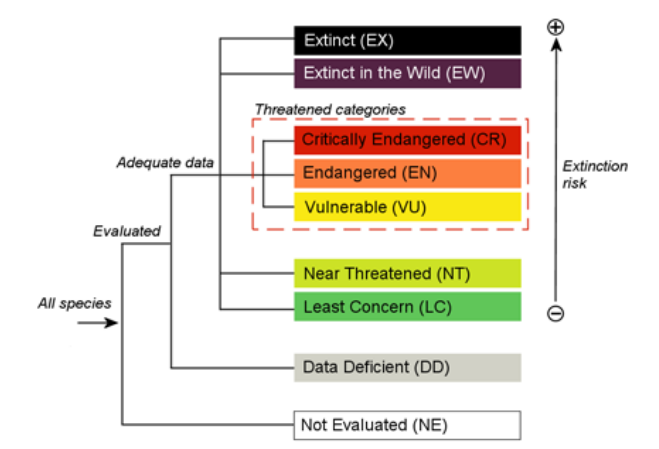
\includegraphics[width=0.35\textwidth]{Images/RedListCategories.png}
	\caption{IUCN Red List categories \\  \autocite{IUCN2000} }
	\label{IUCNcategories}
	
\end{wrapfigure}


\subsection{Why fish?}

The group considered in this study are the \(Actinopterygii\), commonly 
known as the ray-finned fish. Actinopterygii are the largest class of 
vertebrate, with over 33,000 constituent species, with more species being 
described regularly \autocite{Fishbase}. For 
context, mammals are thought to have closer to 6,400 extant species 
\autocite{Mammal2020}; reptiles have 9,500 species 
\autocite{Pincheira-Donoso2013}
; and birds have around 18,000 \autocite{Barrowclough2016}. Unfortunately, the 
Actinopterygii are also proportionally 
the most understudied class of the vertebrates. for example, just over 50\% 
of Actinopterygii are assessed in the IUCN Red List, 
compared with the 62-90\% of other classes, as laid out in 
Table ~\ref{ClassAssessment}. \\

	\begin{tabular}{lrrr}
	\textsc{Class} & \textsc{\# of Species} & \textsc{\# Assessed} & \textsc{\% 
	Assessed} \\	
	\hline
	\textsc{Actinopterygii}	& 33,000 & 17,955 & 54.4 \\
	\textsc{Mammalia} & 6,500 & 5850 & 90.0 \\
	\textsc{Aves} & 18,000 & 11,147 & 62.0 \\
	\textsc{Reptilia} & 9,400 & 7892 & 84.0 \\  CHANGE TO BE SQUAMATES
	\textsc{Amphibians}
	\multicolumn{4}{l}{\caption{Table ~\ref{ClassAssessment}: IUCN 
	Red List  assessments for vertebrate classes}} \\
	\multicolumn{4}{l}{ \autocite{Mammal2020, Pincheira-Donoso2013}} \\
	\multicolumn{4}{l}{ \autocite{Barrowclough2016, Fishbase}}
	\label{ClassAssessment}
	
\end{tabular}
\newline
\newline

The IUCN is not the only research body in which Actinopterygii are poorly 
represented. A 
quick search in WebofScience also demonstrates the lack of research into this 
class. When searching for topics that include the class names of the groups 
mentioned in Table ~\ref{ClassAssessment}, the results are as follows: 
Actinopterygii -2055; Mammalia - 8905; Reptilia - 6,030; Aves - 13,116.  This 
bias is acutely present in conservation science - a recent study by 
\cite{Watson2017} revealed that, of the vertebrate groups, fish had the highest 
imbalance between number of published studies and number of described species 
(16\% and 50\% respectively).

Despite the lack of studies into Actinopterygii, many species of fish are 
acknowledged to be very important as a source of food and employment - through 
fishing, tourism and entertainment. Fish consumption 
has been rising steadily for the past 6 decades, as highlighted clearly in 
Figure ~\ref{GlobalCatch}. 

\begin{wrapfigure}{r}{0.5\textwidth}
	
	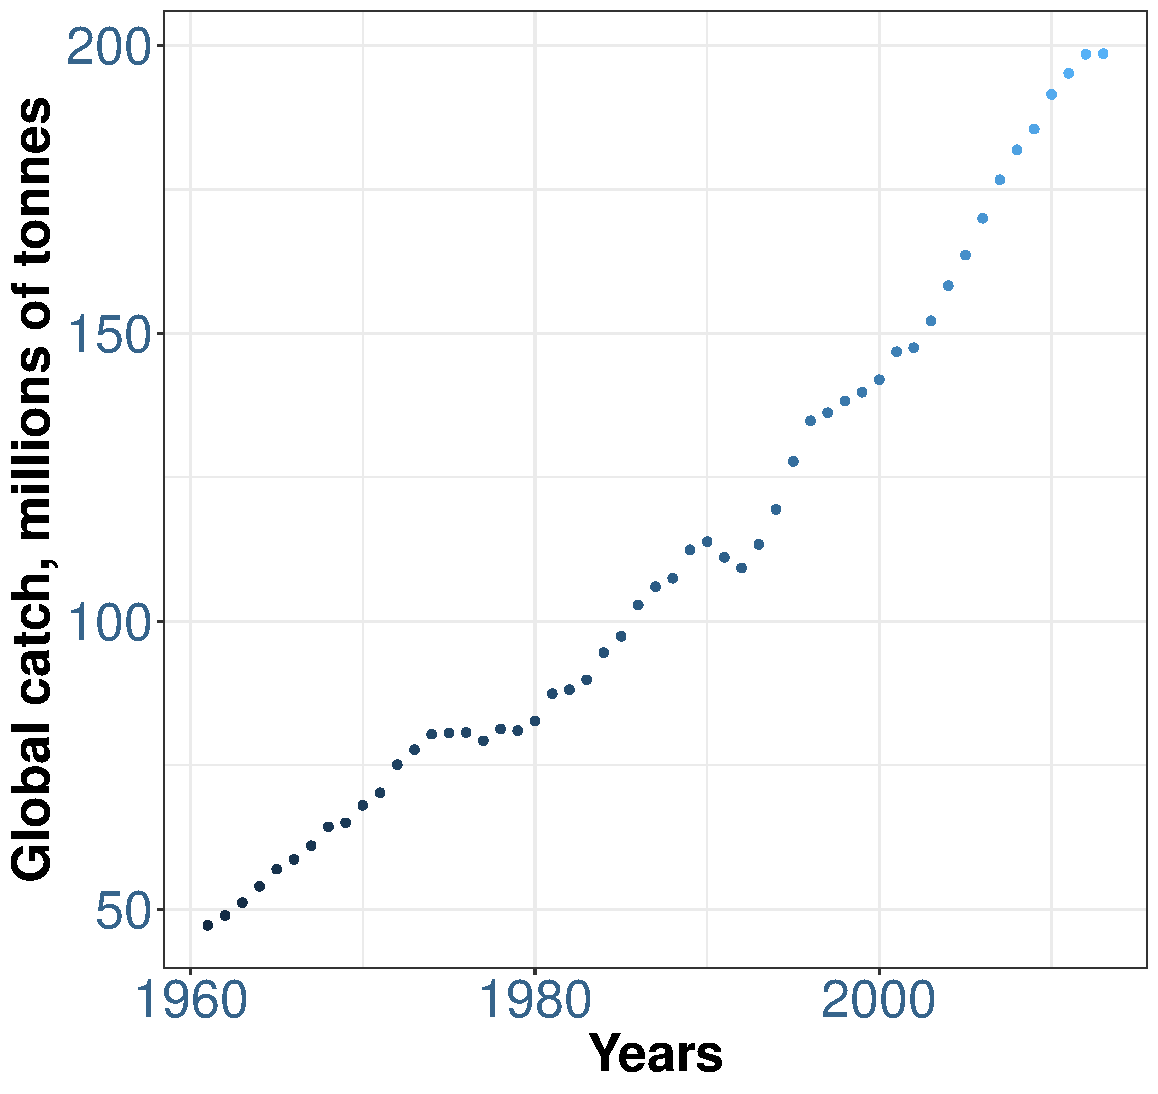
\includegraphics[width=0.4\textwidth]{Images/GobalCatch.pdf}	
	\caption{Global catch of freshwater, demersal, pelagic and marine fish, \\
	\autocite{FAO2020} }  
	\label{GlobalCatch}
	
\end{wrapfigure}


Many people, especially in Europe and Northern 
America, are increasing the amount of fish in their diet - some to improve 
their health 
\autocite{Rimm2006}), and others to 
lessen their impact on the environment \autocite{Mary2020}. Younger generations 
are particularly aware of the impact their food choices have on the planet 
\autocite{Mary2020}, so it could be assumed that this trend of eating more fish 
is unlikely to change. This increased demand for fish (and fish-related 
products) has lead to an increase in aquaculture (farming fish) 
\autocite{Belton2018}. Wild-caught 
fish number are in decline due to stock exhaustion and 
populating collapse rather than a decrease in interest in wild caught fish 
\autocite{Tremblay2011, Belton2018}. 

Marine ecosystems in particular are under increasing pressure from human 
action. Globally, governments and scientific bodies have agreed that ecosystems 
need to be protected in order to protect the future of marine resources 
\autocite{MurakiGottlieb2018}. Marine Protected Areas (MPAs) are one such form 
of 
protection - 
however the definition of these vary significantly from one location to 
another \autocite{Marinesque2012}. In general, an MPA's success is evaluated by 
its effectiveness at conserving 'keystone' species, or their value to local 
fishing activities \autocite{Marinesque2012}. As discussed above, by 
considering only 'keystone' species, considerable ecosystem damage may occur 
un-measured, and many species may go un-protected. 

Given that many species of fish 
exist in both the marine and freshwater realms, and many more migrate around 
the globe, clear conservation prioritisation for fish will be crucial to ensure 
we do not fail to protect vulnerable and non-charismatic species. 


\subsection{X, Y  and Z}
subsection: why these fish in particular



[now to sum everything up] \\

It is clear that the Actinopterygii group is both under-studied and 
under-protected, despite their importance to human populations across the 
globe. This study is a first step in directly addressing this imbalance. Using 
the EDGE metric, we create conservation prioritisation lists for [X, Y and Z] 
and, along with geospatial analysis of their current habitats and threats, 
highlight methods through which vulnerable species could be protected. This 
study also provides a roadmap that will be useful for the creation of reports 
regarding other family groups within the Actiopterygii class.  





	\section{Methods}
	\noindent

\subsection{Taxanomic Matching}

\subitem{Data Collection}


# JUST INCLUDE FISH in detail
# mention other taxanomic 
# include versions of data 
# source for other trees from Rikki 

Before performing the EDGE2 analysis, I needed to create the most up-to-date 
species list of each taxanomic group, source a phylogenetic tree set, and then 
adjust the species in the tree according to the latest species list. 

Of the vertebrate groups that I calculated EDGE for, Birds, Squamates and 
Amphibians had already gone through the process of taxanomic matching and 'tree 
cleaning'. Chondrichythes, Actinopterygii, Mammals and Agnatha all required 
this process.

The first step was to establish a taxanomic authority. For Mammals we used the 
data from 'VertLife'\autocite{}, which pulls taxaonomic data from the ASM 
Mammal Diversity Database. For Condrichythes, Actinopterygii and Agnatha, we 
used FishBase as the taxanomic authority \autocite{Fishbase} . This means that 
we used the species data from this group, and adjusted species names in our 
other data sources to match the authority. 

The second data set we require was a phylogenetic tree/ set of trees. Each of 
these data came from a specialised site. For the Actinopterygii class we used 
the set of 100 trees from \cite{Chang2019}. For the Chondrichthyes 
we used the trees from INSERT SHARK TREE SOURCE. For Mammals we used the tree 
set from HERE. For the Agnatha [insert what actually happened when I do this 
piece of work].

The third data set we used was the IUCN Red List, as the probability of 
extincion (pext) value is calulcated based on the Red List "Extinction" 
Category \autocite{IUCN2000}.

To create the 'master species' list the first step was to strip out any 
sub-speciies from the master species list - this was done by removing any data 
entries with three componants i.e. [example]). We then compared the list of 
species in the phylogenetic trees and in the Red List data 
with the taxanomic authority. For any species that were in the trees or in the 
red list that weren't in the taxanomic authority, we manually checked to see if 
these species were either spelling mistakes or synonyms of valid species. If 
the species was an incorrect spelling of a valid species, then the name was 
corrected. If the species was a synonym of a valid species, then the database 
was checked to see if the correct species was in the database. If it was not, 
then the name was changed to the valid species name. If the valid species was 
also present in the database, then the species was discarded.  If the species 
was neither a spelling mistake nor a synonym, then it was also discarded. 
[Create a diagram for this?]

At the end of the taxanomic matching, we had a data frame for each taxanomic 
group containing the taxanomic species name, genus and family, the tree 
species, and the red list category (n.b. the tree species and red list category 
were entered as NA if the valid species weren't found in the tree or evaluated 
by the red list).

We then updated the phylogenetic trees. Using a base set of 1000 trees, we 
removed all of the species in the tree that were not in the taxonomic database 
(the 'invalid' species). We then checked to see if there were any family groups 
that were missing from the tree, and imputed a single species from each family 
group. We repeated this with the genera. Then, we imputed the rest of the 
missing species. As the imputation process is somewhat random, the result was 
1000 unique trees for each taxanomic group. 


\subsection{EDGE, EDGE2 and PD calculations}

Once we had all of the updated phylogenetic trees and IUCN data we looked at 
EDGE2 scores and phylogenetic diversity loss across the whole taxanomic tree 
for each of our clades. The EDGE2 metric is an updated way version of the EDGE 
metric, originally designed by \cite{Steel2007}.

How to calculate EDGE scores: 

How to calculate EDGE2 scores: 

How to calculate PD loss: 

## advice from Rikki: 	

call it ePD loss and link to \autocite{Faith2008} and \autocite{Steel2007}


For each of the vertebrate groups we:
-Calculated EDGE2 (individual speices ePD score) Scores using 7 pext values* 
(including clade-specific where 
possible)
-- Did a spearman analysis of the top 100 EDGE species in each pext forecast
to see if the  pext forcast affects the EDGE ranking
- Calculated EDGE scores for fish - 
-- did a spearman anaylsis of the top 100 EDGE species with the top 100 EDGE2 
species for each forcast
-Calculated percentage PD loss for each clade using the 7* pext values 
(*including clade-specific wehre possible)


--- FOR JUST FISH OR FOR ALL VERT GROUPS? 
- Scrambled pext (for all 6 pext forcasts) and calculcated percentage PD loss. 
-- Do some kind of analysis to see if there is a difference between the PD loss 
in the switched up data and the correct data set. 


\subsection{Clade selection}

We picked three clades for the in-depth threat analysis. To pick the most 
suitable clades we first screened each family group for size, Red List coverage 
and presence of vulnerable species. We then created super-family clusters of 
families that: had >50\% Red List Coverage and at least 1 vulnerable species, 
>100 species, and were monophyletic. 
This left us with 21 large clusters (is this for the results section?) [have 
table with all of the groups in??]. We then 
looked into each of these clades to find if there were any biological meaning 
to these clusters of family groups. This left us with XXXX groups.
We then picked 3 final groups for [x y z reasons]. 

 

\subsection{Clade threat analysis}

For the selected clades we:
- Produced an EDGE list, using the EDGE 2 metric. 
- Threat analysis
- Range analysis
- Overlap with MPAs? Especially of important areas?
- Trends in threat? Increasing/ decreasing/ static?





\subsection{Packages and technical specifications}

rfishbase
rredlist	
phylbase
capter
phytools
data.table
geiger
pez


\section{Results}
\noindent

\subsection{Updated phylogenetic trees}
SHOULD I TALK ABOUT HOW MANY SPECIES I NEEDED TO IMPUTE for each taxanomic 
group? 
yes - but briefly. Add a table showing everything I did. 

image: fish tree as a fan coloured by red list category OR by ED: look at 
phytools blog 


\subsection{PD loss}

Insert: image with percentage PD loss across 6 vertebrate groups with all 6 
pext forecasts
- maybe only show 3 pext 
Insert: Tree showing the evolutionary relationship of the 6 vertebrate groups.
fish in colour, rest in gray, using silouettes of the orGANISMS) 

\subsection{PD at threat: random or not}
Insert: barplot showing range of PD loss with real data vs scrambled, plus an 
analysis to see if there is a statistical difference. 

\subsection{EDGE1 vs EDGE 2}
Insert: eeither multi-panel of the spearman analyses of the EDGE 2 vs EDGE 1 
scoers for all vertebrate groups, or just pick one/ two (dpeending on results) 
and descript. 

\subsection{EDGE 2 - variation by pext}
Insert: show image from spearman analysis comparing top 100 across all of the 
EDGE 2 groups. 
- NOT SURE IF NEED A PLOT, MAYBE JUST DISCUSS: PERCENTAGE OVERLAP OF THE TOP 100


\subsection{EDGE RANKING}
TABLE OF TOP 20 SPECIES 




\subsection{THREAT analysis}
Something about threats. 



\section{Discussion}
\noindent



%	\section{References}
\noindent
\printbibliography 


\section{Appendix: Supplementary materials}

	



\end{document}